\documentclass[12pt,a4paper]{report}
\usepackage[utf8]{inputenc}
\usepackage{amsmath}
\usepackage{amsfonts}
\usepackage{amssymb}
\usepackage{graphicx}
\usepackage{listings}
\usepackage{fancyhdr}
\usepackage{parskip}
\usepackage{rotating}
\pagestyle{fancy}
\chead{2.1.10 - sw608f14 - Daniel S. F., Lars A, Mathias W. P. \& Søren S. A.}

\lstset{mathescape = true}
\usepackage{amsthm}
\begin{document}
\section*{Selfstudy 3}
\section*{1.}
This exercise has been answered in the last selfstudy.
\section*{26-1 Escape Problem}
\subsection*{b}
Part a greatly hints how to model a flow network.
Here is an example of a grid's (3x3) corresponding flow network, figure \ref{diagram}, where (1,1) and (2,2) are marked, with the answer to part one this can then be made into a regular flow network.

\begin{figure}[h]
     \centering
     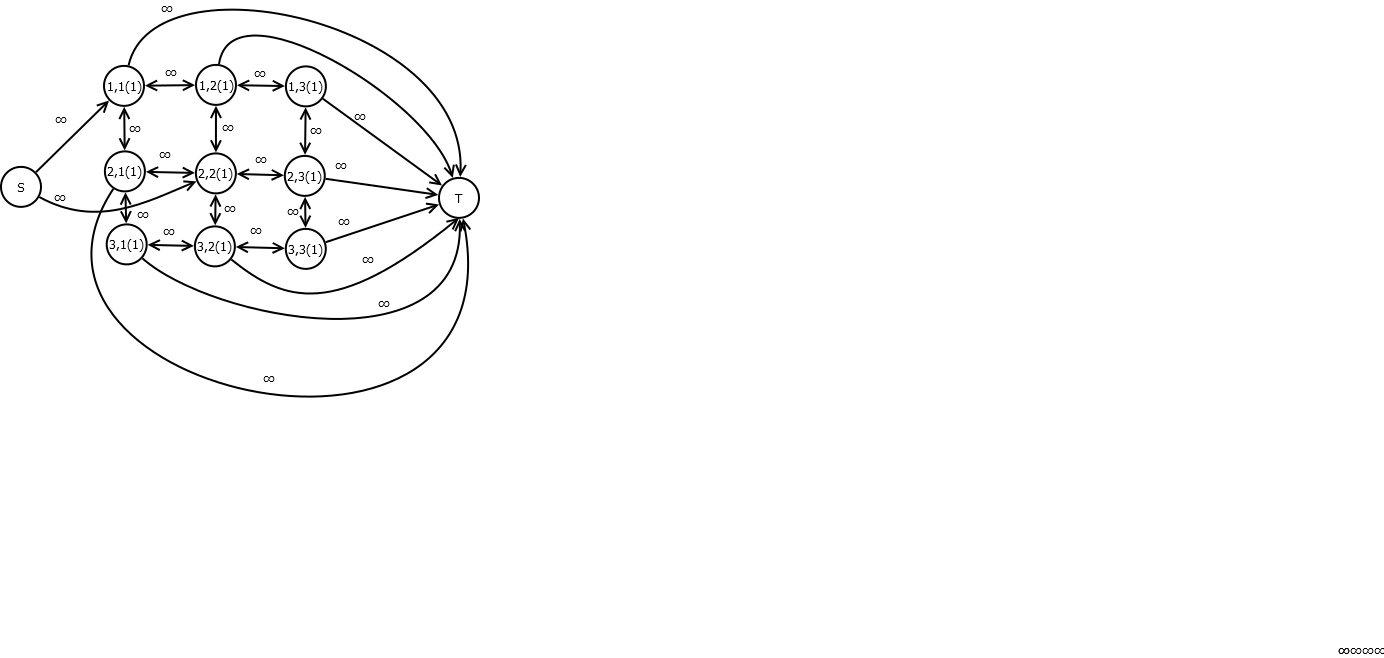
\includegraphics[scale=0.5]{diagram}
     \caption{Diagram of flow network.}     
     \label{diagram}
     
\end{figure}

How the flow network will be constructed is as follows.
We very much follow figure 26.8
One source node S and a target node T is added.
Furthermore there is an edge for each field in the grid, named $v_{i,j}$. 
Each $v_{i,j}$ has weights 1 (which can afterwards be transformed into a regular flow network), and is connected to its adjacent vertices in both directions with flow 1.
S gets assigned an edge of flow $\infty$ to each start node.
Furthermore from each vertice $v_{i,j}$ where it is a border vertice, it will have an edge going from it to T with $\infty$ flow.
Then when the network has been converted to a flow network, it is just a matter of running Edmond Karp from S to T and see whether the flow reaching T is lesser or greater than $m$.
Its running time is then $O(V^2E$) as constructing the network could be done in linear time.

\section*{17-2}
\subsection*{a.}
For search, the problem will consist of searching in the arrays $A_i$ where $n_i = 1$.
A search that can be used is binary search.
Here is an analysis of its worst case running time.
$$\sum\limits_{i=0}^{k-1} lg(2^i) = \sum\limits_{i=0}^{k-1} i = \frac{1}{2} * (k-1) * k = O(k^2) = O((lg(n+1))^2) = O(lg(n)^2)$$

\subsection*{b.} 
\end{document}